\documentclass{standalone}
\usepackage[utf8]{inputenc}
\usepackage{newtxtext}
\usepackage{newtxmath}
\usepackage[italic]{hepnicenames}
\makeatletter\def\@shiftlen@anti@gen@bar{0mu}\makeatother
\usepackage[svgnames]{xcolor}
\usepackage{tikz-feynhand}


\begin{document}
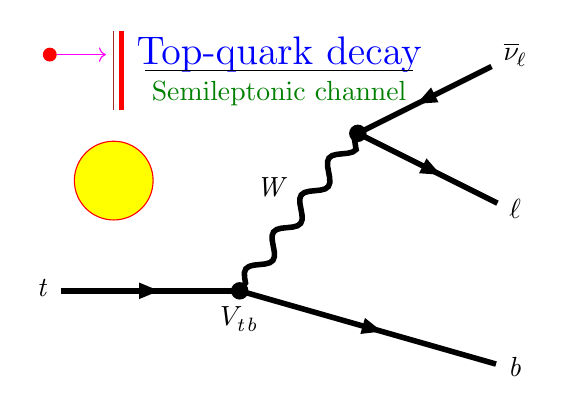
\begin{tikzpicture}
  \setlength{\feynhandlinesize}{2.0pt}
  \tikzfeynhandset{every fermion={/tikz/color=Black},}
  \tikzfeynhandset{every boson={/tikz/color=Black},}
  \tikzfeynhandset{every dot={/tikz/color=Black},}
  \begin{feynhand}
    \node at (0.0, 4.0) {\textcolor{Blue}{\Large Top-quark decay}};
    \vertex [particle, Black] (t) at (-3.0, 1.0) {\Ptop};
    \vertex [particle, Black] (b) at (3.0, 0.0) {\Pbottom};
    \vertex [particle, Black] (l) at (3.0, 2.0) {\color{Black}\Plepton};
    \vertex [particle, Black] (nu) at (3.0, 4.0) {\APnulepton};
    \vertex [dot, Black, label=below:\color{Black}\(V_{\Pqt{}\Pqb}\)] (tb) at (-0.5, 1.0) {};
    \vertex [dot, Black] (Wlnu) at (1.0, 3.0) {};
    \propagator [fermion, Black] (t) to (tb);
    \propagator [fermion, Black] (tb) to (b);
    \propagator [boson, Black] (tb) to [edge label={\PW}, color=Black] (Wlnu);
    \propagator [fermion, Black] (Wlnu) to (l);
    \propagator [fermion, Black] (nu) to (Wlnu);
    \node at (0.0, 3.5) {\textcolor{Green}{Semileptonic channel}};
    \vertex (FHTb0) at (-1.7, 3.8); \vertex (FHTe0) at (1.7, 3.8);
    \draw (FHTb0) to (FHTe0);
    \vertex (FHTb1) at (-2.0, 4.3); \vertex (FHTe1) at (-2.0, 3.3);
    \draw [Red, line width = 2pt] (FHTb1) to (FHTe1);
    \vertex (FHTb2) at (-2.1, 4.3); \vertex (FHTe2) at (-2.1, 3.3);
    \draw [Brown,] (FHTb2) to (FHTe2);
    \vertex (FHTb3) at (-3.0, 4.0); \vertex (FHTe3) at (-2.2, 4.0);
    \draw [Magenta,{Circle[Red, width=5pt, length=5pt]}->,] (FHTb3) to (FHTe3);
    \filldraw[fill=Yellow, draw=Red] (-2.1,2.4) circle [radius=0.5cm];
  \end{feynhand}
\end{tikzpicture}
\end{document}
